\documentclass[letterpaper]{article}
\usepackage{natbib,alifexi}
\usepackage[bordercolor=gray!20,backgroundcolor=blue!10,linecolor=blue,textsize=footnotesize,textwidth=0.8in]{todonotes}
\usepackage{hyperref}
\usepackage{algpseudocode}
\usepackage{algorithm}
\usepackage{subfig}

\title{Implementation\\Playing FPS Games with Deep Reinforcement Learning}
\author{Titouan Christophe$^{1}$, Florentin Hennecker$^{2}$, Nikita Marchant$^{1}$ \and Bruno Rocha Pereira$^{1}$ \\
\mbox{}\\
$^1$Vrije Universiteit Brussel, Pleinlaan 2, 1050 Brussels, Belgium \\
$^2$Universit\'e Libre de Bruxelles, Boulevard du Triomphe - CP 212, 1050
Brussels, Belgium \\
tichrist@vub.be, fhenneck@ulb.ac.be, \{nimarcha,brochape\}@vub.ac.be}

\marginparwidth=0.5in
\newcommand\Tstrut{\rule{0pt}{2.6ex}}
\newcommand\Bstrut{\rule[-0.9ex]{0pt}{0pt}}


\begin{document}
\maketitle

\begin{abstract}
In this article, we study a Deep Recurrent Q-Learning Network implementation
playing in the DOOM video game. Our findings are based on a publication from
\cite{Lample2016}. We first present deep Q-learning under two variants (DQN and
DRQN) which were applied to video games. We then present how we built our own
implementation of a testbed for such algorithms. Finally, we present our results
on a simplified game scenario.
\end{abstract}

\section{Introduction}
Deep Q-Learning is a technique which combines the Q-Learning algorithm with
a deep neural network. In this particular architecture, the expected return of
each action is predicted by a neural net. The agent using this algorithm then
chooses the best action based on a policy (we only used $\epsilon$-greedy here).
Neural networks, particularly convolutional neural networks, are very good at
encoding a highly dimensional state (in this case, a 108x60 RGB image) into a
meaningful lower dimensional state. Moreover, a recurrent neural network can
help handle the sequential nature of playing a video game by passing a hidden
state from one frame to the next.
\todo{find good refs for claims on NN}.

In order to plug our work to the DOOM game, we are using the ViZDoom environment
\citep{Kempka2016} that provides a programming interface to interact with a
DOOM game in various languages (we use Python). ViZDoom provides access to the
screen buffer and actions buttons, as well as game meta-data (such as player
position and the labeled objects in the field of view), used only at training time.

Our agent plays the basic scenario, where he is in a rectangular room.
At the beginning, the enemy spawns at a random position on the opposite side of
the room. The game ends if the agent kills the enemy, or if 500 game ticks elapsed.

\section{Method}

\subsection{Background} We will give in the paragraphs hereinbelow a state of
the art of the technologies that we used in our implementation. We first present
the Deep Q-Learning Network from DeepMind, then its variant Deep Q-Learning
Recurrent Network.

\subsubsection{Deep Q-Networks}
Many reinforcement learning problems have a very high-dimensional space-state
in which each dimension on its own bears very little information. Approximating
a state-action $Q$ function over all possible states and actions becomes quickly
intractable. However, deep neural networks have an outstanding capability to
encode high-dimensional states into a meaningful lower-dimensional hidden state;
moreover, they are also known for their function approximation capabilities
\citep{Hornik1991}. Deep Q-Learning \citep{Mnih2015} is a major breakthrough
showing that neural networks can learn to play Atari games.

In the context of a Deep Q-Network (DQN), an agent tries to learn
$Q(s_t,a_t)$ which represents an
estimation of how valuable an action $a_t$ is in a state $s_t$. In order to
find $Q^*$, the optimal $Q$-function, DQNs use a neural network
parametrized by $\theta$, which represents the weights of the neural network
and gives an approximation called $Q_\theta$ further in this paper. Their goal
is to find the optimal and real $Q$-function $Q^*$ which is verifies the Bellman
optimality equation:
$$ Q^*(s,a) = E\{r + \gamma \max_{a'}Q^*(s',a')|s,a\} $$
With $r$ being the reward of playing $a$ in a state $s$, $\gamma\in [0,1]$ the
discount factor and $(s',a')$ being the next state and its associated action

This gives, since $Q_{\theta} \approx Q^*(s,a)$ the loss function below:
$$ L_\theta(\theta_t) = E_{s,a,r,s'}\{(r +\gamma \max_{a'}Q_\theta(\theta_t)(s' , a' )-Q_{\theta_t}(s,a))^2\}$$

This loss is computed on uniformly sampled game transitions stored in a
replay memory instead of the previously played transition to reduce correlation
between samples. Algorithm \ref{dqn} shows how a Deep Q-Network is trained.
\begin{algorithm}
\caption{The DQN training algorithm}\label{dqn}
\begin{algorithmic}[1]
	\For{number of episodes}
		\State{create new episode}
		\While{episode not finished}
			\If{random() $\leq$ epsilon}
				\State choose random action
			\Else
				\State choose action with highest Q
			\EndIf
			\State store old state, action, new state and reward in memory
		\EndWhile
		\For{number of back-propagation steps}
			\State update Q-network with a batch of random sequences
		\EndFor
	\EndFor
\end{algorithmic}
\end{algorithm}


\subsubsection{Deep Recurrent Q-Networks}
One of the issues posed by the model described above is that it assumes that the
environment is fully observable. However in the case of DOOM, we only get a
partial
observation of the environment, limited by the field of vision of the main
character. Previous ways of solving that issue have been to feed a sequence of
frames to the DQN as a history.
A potentially better way to solve the history issue is to use a Deep Recurrent
Q-Network, as described in \citep{Hausknecht2015}. A DRQN
estimates $Q(s_t,h_{t-1},a_t)$ instead of the regular $Q(s_t,a_t)$. The
parameter $h_{t-1}$ represents the hidden state of the agent at the previous
transition. In our case, we will use a Long Short-Term Memory layer (LSTM)
\cite{Hochreiter1997}. In addition to the input and output state of usual neural
networks, a LSTM unit also carries a hidden state, which has to be fed along
with the input, and retrieved with the output. This hidden state is able to
convey information about patterns that evolve along time. In our case, it is
expected to carry information on portions of the game that have been observed
but which are no more visible.

\subsection{Model details}
Our neural network is the same as the one presented in \citep{Lample2016},
with one addition.
It is composed of two convolutional layers followed by three separate
sub-networks. One of these sub-networks is used in a supervised manner to
predict various game features (see below), the second is a standard
DRQN network while the last is a standard DQN output. The network is trained
with or without the game features and with either the DRQN or the DQN output.
The hidden size of the LSTM was set to 300 units.

\begin{figure*}[h]
  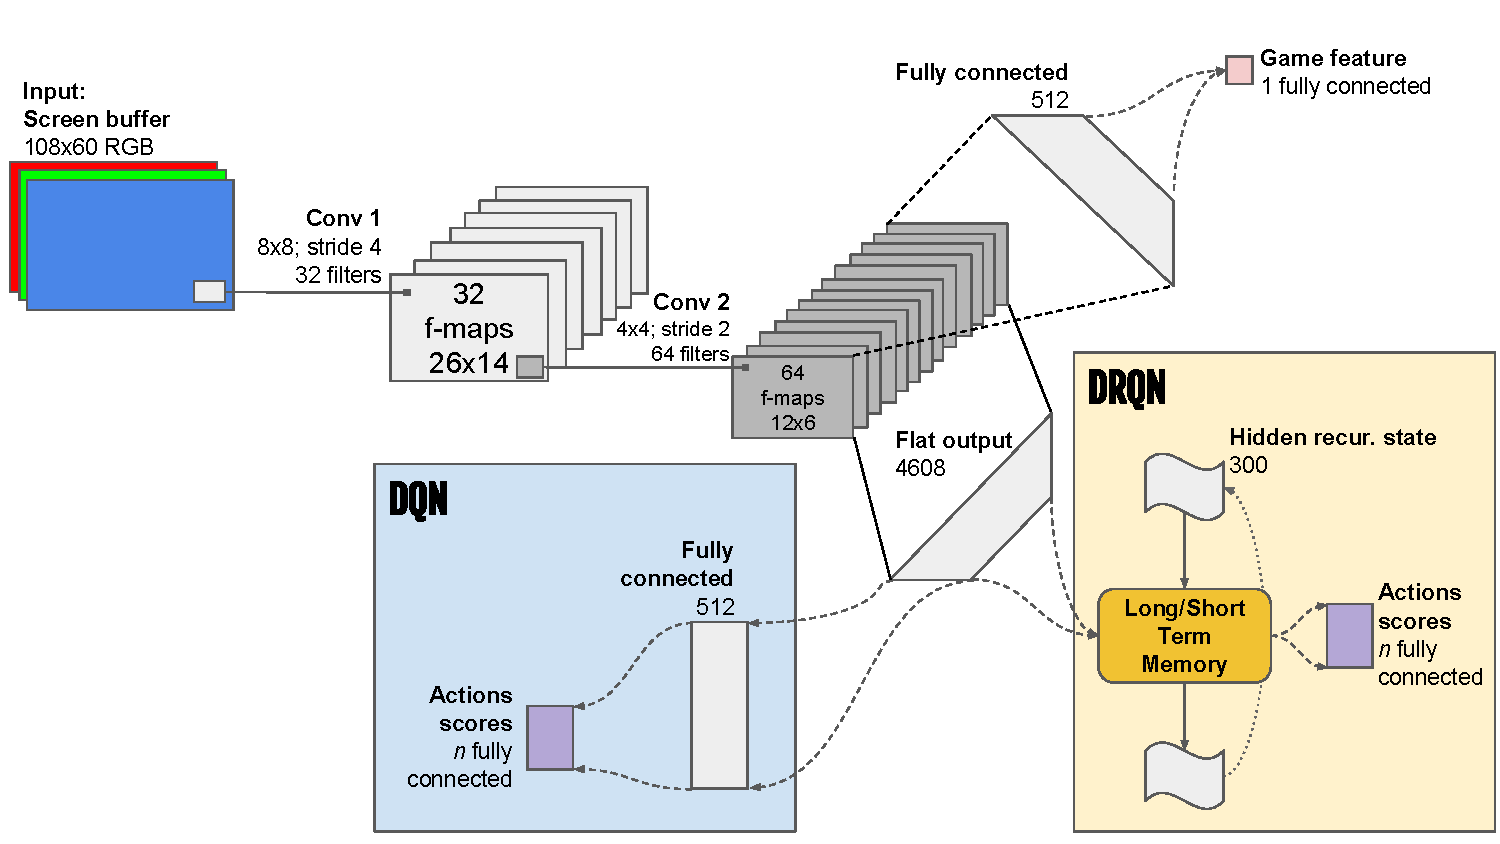
\includegraphics[width=\textwidth]{DRQNSchema.pdf}
  \caption{\label{fig:drqn-schema} Our network and its variations}
\end{figure*}



\subsubsection{Game Features} As described in the paper \citep{Lample2016},
agents not using the game features were unable to accurately detect enemies and
were thus randomly shooting around hoping that those shots would reach their
targets. In order to make up for a lack of efficiency, we used custom made game
features to train the agent in a supervised setup jointly with the Q-learning
setup to tell the agent if enemies were in his field of vision.  The
\texttt{Label buffer} provided by the Vizdoom API  was used to fetch all the
entities present in the vision frustum. However, entities hidden by other scene
elements, typically walls, were also parts of that buffer. We then used the map
characteristics in order to to check if an entity was visible or not. Even
though this information can't be used during testing phase, it was used during
the training of the agents to improve their accuracy. We also created a game
feature estimating the lateral position of an enemy against a wall in a much
simpler DOOM map.

\subsubsection{Frame Skip}
To reduce the computational complexity, it is common to use the skip-frame
technique. With this technique, the agent receives a input frame every $k + 1$
game frames, where $k$ is the number of of frames skipped. During those
skipped frames, the last action of the agent is repeated automatically.
We used a value of $k=4$ because it is a good trade-off between
computing performance and agent accuracy \citep{Kempka2016}.


\subsubsection{Sequential Updates}
When training an LSTM, one feeds sequences of data for which the LSTM will
predict one output per time step. However, the LSTM will zero its hidden state
before the start of each sequence, and it will take several time steps for the
hidden state to initialize. Hence, the outputs for the first time steps might
be erroneous since their previous hidden state was not fully initialized.
To solve this, we discard the first time steps outputs when computing the loss,
as explained in \citep{Lample2016}.

\subsubsection{Hyper-parameters}
Analogously to \cite{Mnih2015} and \cite{Lample2016}, we use a replay memory
size of $1000000$ frames. The sequence length of
the training samples was set to 8, but only the last 4 outputs were accounted
in the loss.
Each frame consists of a 8 bit per color \texttt{RGB} buffer of dimension
$108 * 60$\footnote{As VizDoom does not support natively this resolution, we
used the $200 * 125$ resolution and downsampled it before feeding it to the
agent.}.
In the bootstrapping phase, our agent only plays random actions drawn from the
set \texttt{TURN\_LEFT, MOVE\_LEFT, MOVE\_FORWARD, JUMP, MOVE\_RIGHT}. We do
not add the \texttt{TURN\_RIGHT} and \texttt{MOVE\_BACKWARD} actions, because
a uniformly random sample of all these actions would lead the agent to stay
at the same place and face approximately the same direction all the time. This
bootstrapping phase is used to populate the replay memory. Once the
bootstrapping phase is over, we run algorithm \ref{dqn} with $\epsilon$ starting at
1 and decreasing linearly to 0.1 over 4000 episodes.

We used the RMSProp \citep{rmsprop} algorithm with a learning rate of 0.001.

\subsubsection{Dropout}
Dropout \citep{Srivastava2014} was added to the fully connected layers, with
a probability of keeping each unit of 75\% at training time.

\subsection{Action phase}
As opposed to the paper \citep{Lample2016} which uses a navigation phase as
well as an action phase, we decided to only focus on the action phase. The
navigation phase is the phase where the agent focuses on exploring the map to
collect items and find enemies. We indeed dropped that step to immediately
concentrate our efforts on the action phase, which consists in shooting at
enemies when they are detected. This so-called action phase will of course
take place after a training phase during which the agent learns how to interact
properly with the game.

\subsection{Limitations} In order to train and test our implementation, we only
used one simple single-player scenario. It consists of a square room with one
enemy in front of and visible by the agent. The scenario ends when the agent
manages to kill the enemy or when the timer reaches 0. This means that we have
in that case a fully-observable environment.\todo{}

\subsection{Implementation}
We implemented the model using Python 3 and Tensorflow \citep{tensorflow}.
It is available publicly on Github
\footnote{\url{https://github.com/fhennecker/deepdoom}}.



\section{Results}
% Notes:
% Fully Observable Markovian Process (FOMP): basic with MOVE_LEFT, MOVE_RIGHT, ATTACK
% * Experiment: e-Greedy decreasing from 1 to 0.1 over 4k epochs, then up to 8k epochs with e=0.1
%               Test with and without game features
%               Test DQN and DRQN
% Partially Observable Markovian Process (POMP): basic with TURN_LEFT, TURN_RIGHT, MOVE_FORWARD, ATTACK
% * Experiment: e-Greedy decreasing from 1 to 0.1 over 8k epochs, then up to 15k epochs with e=0.1
%               Test with DRQN and DQN
%   -> Videos: DQN shoots more often
%
% Quantifiable results (graphs)
% Qualitative results (videos)

\begin{table}[h]
\centering
\begin{tabular}{cc}
\multicolumn{2}{c}{Test Setup}                         \Tstrut\\ \hline
\multicolumn{1}{c|}{CPU} & Intel i7-6800K 3.4 GHz      \Tstrut\\
\multicolumn{1}{c|}{GPU} & Nvidia GeForce GTX 1080 8Go \Tstrut\\
\multicolumn{1}{c|}{RAM} & 32 Go DDR4                      \Tstrut
\end{tabular}
\caption{Test setup hardware specification}
\label{tab:specs}
\end{table}

The training phase as well as the action phase were run on a high-end machine
of which specifications are displayed in Table \ref{tab:specs}.\\

Both DQN and DRQN were run with and without the game feature specifying the
lateral position of the enemy against the back wall of the basic map. Figure
\ref{successrate} compares the rolling proportion of successful episodes
in these 4 settings. The rolling proportion is the number of episodes in which
the agent killed the enemy before the episode ended in the last 64 episodes.

\begin{figure}
	\subfloat[DRQN]{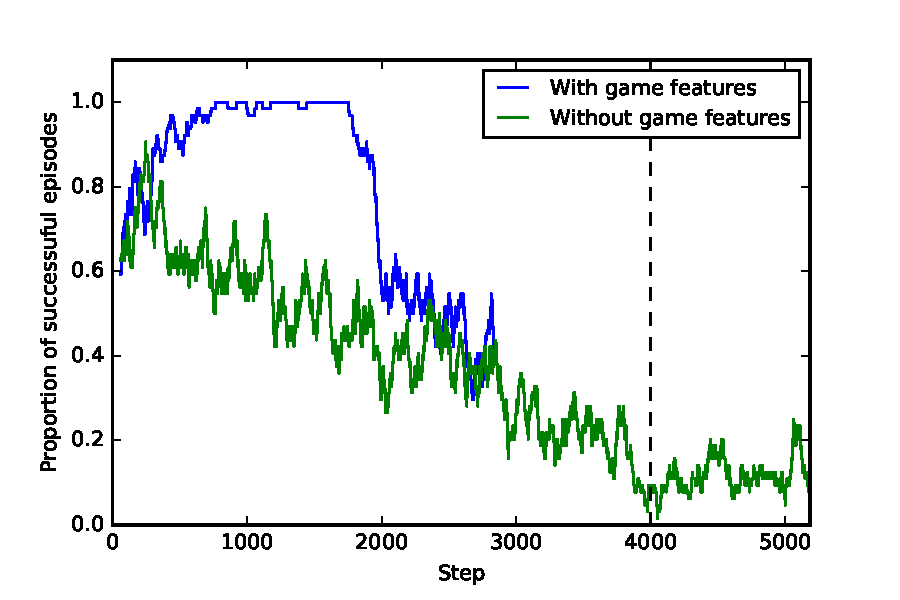
\includegraphics[width=.5\textwidth]{Graphs/success_DRQN.pdf}}\\
	\subfloat[DQN]{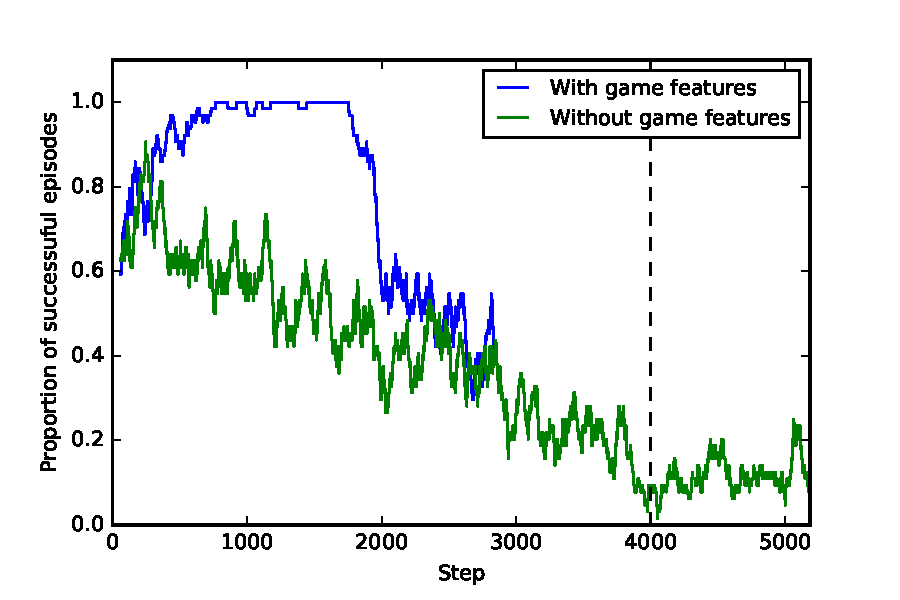
\includegraphics[width=.5\textwidth]{Graphs/success_DRQN.pdf}}
	\caption{Proportion of successful episodes}
	\label{successrate}
\end{figure}

The good performance of DRQN then followed by a sudden drop in performance could
be explained by the fact that $Q$-learning is known to diverge very easily
\todo{ref?}. We can indeed see on figure \ref{averageq} that
even if our agent learns an excellent $Q$-function, its $Q$ values will at some
point start diverging, causing the rolling proportion of successful episodes
to drop significantly. This drop doesn't seem to occur when we remove the
recurrent feedback and use DQN instead.\\

\begin{figure}
	\subfloat[DRQN]{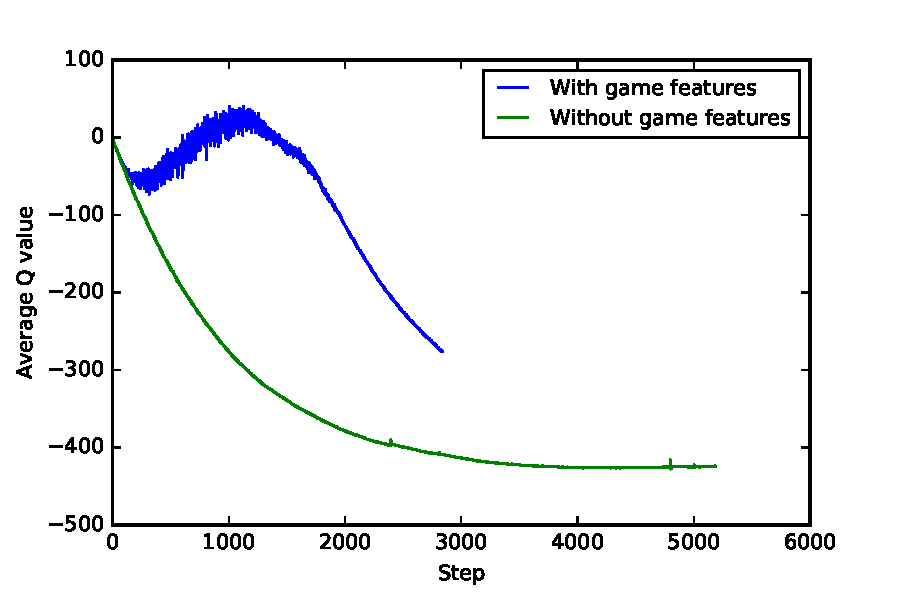
\includegraphics[width=.5\textwidth]{Graphs/qval_DRQN.pdf}}\\
	\subfloat[DQN]{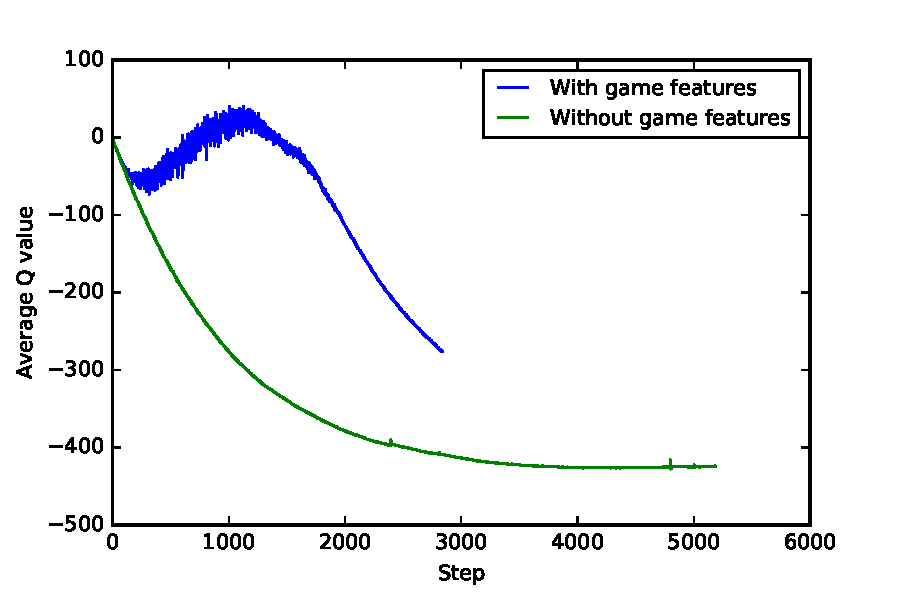
\includegraphics[width=.5\textwidth]{Graphs/qval_DRQN.pdf}}
	\caption{Average $Q$-values}
	\label{averageq}
\end{figure}

Looking at test episodes, the behavior of the agent is excellent (it almost
immediately moves in the right direction then shoots the enemy) until the
$Q$-values diverge at which point the agent will just pick the same action
over and over again; either hugging the left or right wall or shooting
indefinitely without moving.\\
\section{Discussion}


\footnotesize
\bibliographystyle{apalike}
\bibliography{report}


\end{document}
